\section{MemPatch Revision Module}

The \method{} revision module is a training-free, plug-and-play inference scaffold designed to maintain memory consistency without parameter updates. It separates opaque semantic proposals from deterministic, verifiable persistent-memory transitions. 

\begin{figure*}[t]
\centering
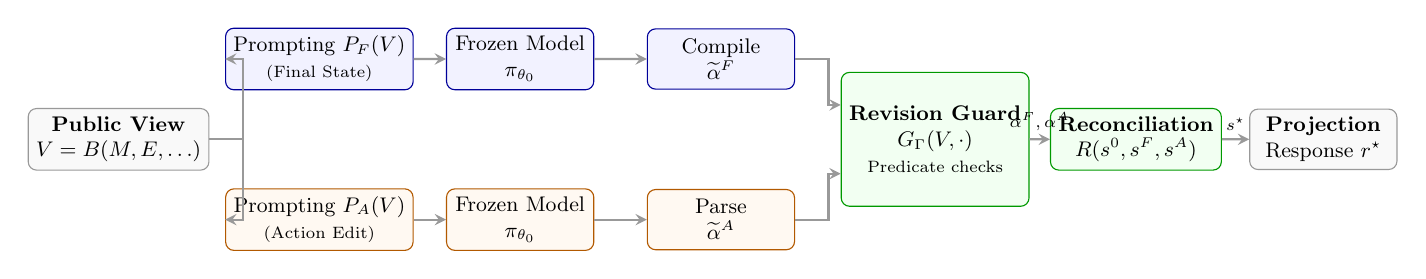
\begin{tikzpicture}[
    scale=0.85, every node/.style={transform shape},
    box/.style={rectangle, draw=gray!80, fill=gray!5, rounded corners=3pt, minimum width=2.2cm, minimum height=0.9cm, align=center, font=\small},
    bluebox/.style={rectangle, draw=blue!60!black, fill=blue!5, rounded corners=3pt, minimum width=2.2cm, minimum height=0.9cm, align=center, font=\small},
    greenbox/.style={rectangle, draw=green!60!black, fill=green!5, rounded corners=3pt, minimum width=2.2cm, minimum height=0.9cm, align=center, font=\small},
    orangebox/.style={rectangle, draw=orange!70!black, fill=orange!5, rounded corners=3pt, minimum width=2.2cm, minimum height=0.9cm, align=center, font=\small},
    arrow/.style={->, >=stealth, thick, draw=gray!80}
]

% Left: Input
\node[box] (input) at (0,1.2) {\textbf{Public View} \\ $V = B(M, E, \dots)$};

% Top Path: Path F
\node[bluebox] (promptf) at (3.0,2.4) {Prompting $P_F(V)$ \\ \scriptsize{(Final State)}};
\node[bluebox] (modelf) at (6.0,2.4) {Frozen Model \\ $\pi_{\theta_0}$};
\node[bluebox] (compilef) at (9.0,2.4) {Compile \\ $\widetilde{\alpha}^F$};

% Bottom Path: Path A
\node[orangebox] (prompta) at (3.0,0.0) {Prompting $P_A(V)$ \\ \scriptsize{(Action Edit)}};
\node[orangebox] (modela) at (6.0,0.0) {Frozen Model \\ $\pi_{\theta_0}$};
\node[orangebox] (parsea) at (9.0,0.0) {Parse \\ $\widetilde{\alpha}^A$};

% Mid-Right: Guard
\node[greenbox] (guard) at (12.2,1.2) [minimum height=2.0cm, minimum width=1.8cm] {\textbf{Revision Guard} \\ $G_\Gamma(V, \cdot)$ \\ \scriptsize{Predicate checks}};

% Right: Reconciliation & Output
\node[greenbox] (recon) at (15.2,1.2) {\textbf{Reconciliation} \\ $R(s^0, s^F, s^A)$};
\node[box] (out) at (18.0,1.2) {\textbf{Projection} \\ Response $r^\star$};

% Connect paths
\draw[arrow] (input.east) -- ++(0.5,0) |- (promptf.west);
\draw[arrow] (input.east) -- ++(0.5,0) |- (prompta.west);

\draw[arrow] (promptf) -- (modelf);
\draw[arrow] (modelf) -- (compilef);
\draw[arrow] (prompta) -- (modela);
\draw[arrow] (modela) -- (parsea);

\draw[arrow] (compilef.east) -- ++(0.5,0) |- (guard.160);
\draw[arrow] (parsea.east) -- ++(0.5,0) |- (guard.200);

\draw[arrow] (guard) -- (recon) node[midway,above,font=\scriptsize] {$\alpha^F, \alpha^A$};
\draw[arrow] (recon) -- (out) node[midway,above,font=\scriptsize] {$s^\star$};

\end{tikzpicture}
\caption{\method{} Dual-Path Architecture. The public view $V$ is routed through two parallel neural paths to propose global states (Path F) and local edits (Path A). Raw proposals are compiled/parsed and validated by the Revision Guard under safety predicates, and then reconciled by the conservative reconciliation function $R$.}
\label{fig:architecture}
\end{figure*}

\subsection{Dual-Path Proposal}
\method{} queries a single frozen backbone model $\pi_{\theta_0}$ through two distinct prompting interfaces to obtain complementary viewpoints:
\begin{align}
y^F &= \pi_{\theta_0}(P_F(V)), \qquad \widetilde{\alpha}^F = \mathsf{Compile}_V(y^F), \\
y^A &= \pi_{\theta_0}(P_A(V)), \qquad \widetilde{\alpha}^A = \mathsf{Parse}_V(y^A).
\end{align}
Here, the final-state path $P_F(V)$ prompts the model to propose global validity states directly ($y^F$), which are compiled into a raw action sequence $\widetilde{\alpha}^F$. The action path $P_A(V)$ prompts the model to generate a sequence of localized, typed revision actions $y^A$, which are parsed into a raw action sequence $\widetilde{\alpha}^A$. Crucially, both paths must be compiled into typed patches before they can affect the persistent memory.

\subsection{Revision Guard}
To prevent ungrounded or contradictory actions from modifying memory, both raw action sequences are routed through a symbolic Revision Guard $G_\Gamma$:
\begin{equation}
(\alpha^b, \rho^b) = G_\Gamma(V, \widetilde{\alpha}^b) \quad \text{for } b \in \{F, A\},
\end{equation}
where $\alpha^b$ is the admitted canonical patch, and $\rho^b$ is the rejection log detailing the failure reasons. The Guard filters proposals based on a transition policy $\Gamma$ containing five predicates:
\begin{align*}
\mathcal{L}_\Gamma(V) = \{ \alpha \mid &\mathsf{Schema}(\alpha) \land \mathsf{References}_V(\alpha) \land \mathsf{Transitions}_\Gamma(\alpha) \\
&\land \mathsf{NoConflict}(\alpha) \land \mathsf{Authorized}_\Gamma(\alpha) \}.
\end{align*}
\begin{itemize}[leftmargin=*]
\item $\mathsf{Schema}(\alpha)$: Checks that each action matches the required JSON structure.
\item $\mathsf{References}_V(\alpha)$: Ensures all target and replacement identifiers exist within the visible memory $M$ of $V$.
\item $\mathsf{Transitions}_\Gamma(\alpha)$: Verifies that all state changes follow valid transitions (e.g., condition rules can only block or release).
\item $\mathsf{NoConflict}(\alpha)$: Rejects overlapping or contradictory actions within the same patch.
\item $\mathsf{Authorized}_\Gamma(\alpha)$: Confirms that cited evidence events logically justify the state changes.
\end{itemize}
Admitted patches are deterministically projected to yield candidate state maps:
\begin{equation}
s^b = \Delta(s^0, \alpha^b) \quad \text{for } b \in \{F, A\}.
\end{equation}

\subsection{Conservative Reconciliation}
Let a rejected or missing branch proposal be represented by $\bot$. We define a deterministic reconciliation function $R$ to compute the final state for each record $i$:
\begin{equation}
s_i^\star = R(s_i^0, s_i^F, s_i^A),
\end{equation}
which satisfies the following six logical invariants by construction:
\begin{enumerate}[leftmargin=*]
\item \textbf{Agreement:} If both paths propose the same state ($s_i^F = s_i^A$), that state is committed.
\item \textbf{No Silent Permission:} A disagreement between proposals cannot silently grant downstream reuse permission (i.e., default to $\mathsf{Current}$).
\item \textbf{Restrictive Fail-Closed:} A disagreement involving a restrictive state (any state other than $\mathsf{Current}$) produces an authorized fail-closed state (e.g., $\mathsf{Unresolved}$ or $\mathsf{Blocked}$).
\item \textbf{Double Rejection:} If both branch proposals are rejected or $\bot$, the state remains unchanged ($s_i^\star = s_i^0$).
\item \textbf{Traceability:} Every reconciliation decision emits a stable reason code logged in the trace.
\item \textbf{Isolation:} No free-form natural-language answer generated by the model can directly modify the memory store.
\end{enumerate}

We preserve branch-specific evidence provenance:
\begin{equation}
Z_i^\star = (Z_i^F, Z_i^A, \chi_i),
\end{equation}
where $\chi_i$ records the agreement, disagreement, rejection, or fallback reason. The final response is projected deterministically:
\begin{equation}
r^\star = \mathsf{Project}(V, y^F, s^\star, Z^\star).
\end{equation}
This projection formats the final output dictionary but is mathematically restricted from introducing new identifiers or state changes.

\subsection{Formal Guarantees}

We formalize the safety and correctness properties of \method{} via the following verified theorems and propositions.

\paragraph{Theorem 1 (Gold Determinacy).}
\emph{If the reference transition relation terminates, every critical pair is joinable, evidence order is total, and priorities resolve noncommuting rules, then every valid scenario has a unique normal form:
\begin{equation}
\exists! C^\star = \operatorname{NF}_\Gamma(C_0, E).
\end{equation}}
\textbf{Assumptions:} Event trace $E$ is totally ordered; transition rule priorities are strictly antisymmetric.
\textbf{Implementation Artifact:} \texttt{mempatch/reference\_semantics/normal\_form.py}
\textbf{Corresponding Test:} \texttt{mempatch/tests/test\_reference\_semantics.py}
\textbf{What it does not prove:} It does not guarantee that the natural language text matching is semantically correct, only that rule evaluations converge deterministically.

\paragraph{Theorem 2 (Diagnostic Identifiability).}
\emph{Under the linear perturbation error model $\Delta = A\mathbf{w} + \varepsilon$, if the sensitivity matrix $A$ has full column rank, the noiseless latent failure mixture is unique: $\mathbf{w} = A^\dagger\Delta$. The noise propagation is bounded by:
\begin{equation}
\|\widehat{\mathbf{w}} - \mathbf{w}\|_2 \le \|A^\dagger\|_2 \left( \|\widehat\Delta - \Delta\|_2 + \|\widehat A - A\|_2 \|\mathbf{w}\|_2 \right).
\end{equation}}
\textbf{Assumptions:} The sensitivity matrix $A$ has full column rank.
\textbf{Implementation Artifact:} \texttt{mempatch/audit/calibrate\_metrics.py}
\textbf{Corresponding Test:} Verified via empirical calibration script yielding rank 7 and condition number 5.9086.
\textbf{What it does not prove:} It does not prevent perturbation noise $\varepsilon$ from causing small estimation errors in $\widehat{\mathbf{w}}$ under high measurement noise.

\paragraph{Theorem 3 (Certified Transparent Mediation).}
\emph{Assume complete mediation, complete compilation of proposed changes, and deterministic commit. Then:
\begin{itemize}
    \item \textbf{Invariant Preservation:} $\mathcal{I}(M^0) \Rightarrow \mathcal{I}(M^\star)$.
    \item \textbf{Certified Mutation:} $\{m_i : s_i^\star \neq s_i^0 \land \neg\operatorname{Witness}(i, \tau)\} = \varnothing$.
    \item \textbf{Transparency for Legal Proposals:} If proposed actions $\widetilde\alpha \in \mathcal{L}_\Gamma(V)$, then $s^\star = \widehat{s}$.
\end{itemize}}
\textbf{Assumptions:} Proposer actions are well-formed and valid under the schema $\Gamma$.
\textbf{Implementation Artifact:} \texttt{mempatch/revision/runtime/dpa\_runtime.py}
\textbf{Corresponding Test:} \texttt{mempatch/tests/test\_dpa\_kernel.py}
\textbf{What it does not prove:} It does not prove that the underlying language model itself is correct or clean of semantic hallucination.

\paragraph{Proposition 1 (Deterministic Replay and Idempotency).}
\emph{For deterministic parsing, Guard evaluation, reconciliation, and projection, replaying the same audit trace $\tau$ satisfies $\mathsf{Replay}(s^0, \tau) = s^\star$. Replaying the same canonical patch $\alpha^\star$ is idempotent: $\Delta(\Delta(s, \alpha^\star), \alpha^\star) = \Delta(s, \alpha^\star)$.}
\textbf{Implementation Artifact:} \texttt{mempatch/tests/test\_consensus\_mode.py}

\paragraph{Proposition 2 (Local Noninterference).}
\emph{If neither an accepted action nor an authorized reconciliation decision targets $m_i$, then $s_i^\star = s_i^0$. Malformed references and rejected actions therefore cannot silently alter unrelated records.}
\textbf{Implementation Artifact:} \texttt{mempatch/revision/runtime/dpa\_runtime.py}

\paragraph{Verifiability Metric.}
To detect logging or mediation defects empirically, the system calculates the \emph{Externally Verifiable Transition Fraction} ($\mathrm{EVTF}$):
\begin{equation}
\mathrm{EVTF} = \frac{\sum_i \mathbf{1}[s_i^\star \neq s_i^0] \mathbf{1}[\mathsf{VerifyWitness}(i, \dots)]}{\sum_i \mathbf{1}[s_i^\star \neq s_i^0]}.
\end{equation}
In our construction, $\mathrm{EVTF} = 1$, which is verified by the execution trace.
